\chapter{Multi-tenancy}
This chapter aims to introduce the concepts and ideas surrounding multi-tenancy and explain why it is relevant or even important to current cloud computing practises.

\section{The Cloud}
Cloud computing is commonly defined as a form of computing where computing resources are shared  in contrast to having local dedicated resources to run applications or services \cite{webopedia}. Walker \cite{GraceWalker} further defines cloud computing as an solution that delivers Information Technology (IT) as a service by using computers to work together and applications to utilise these collective computing power as a single system. 

The creation of a public clouds, which offer cloud solutions to the general public has provided anyone with almost unlimited resources and scalability. Large numbers of companies are shifting to using public clouds instead of maintaining their own datacenters. The large costs advantages resulting from using the public cloud is the primary factor fuelling this shift, allowing stronger competition between companies of all sizes. Although cloud computing is not a new technologies but simply a way computing resources are delivered (much akin to historic mainframes), it is a major paradigm shift in the way information and services are provided \cite{GraceWalker}. All of this has created a need for radical redefinition of our current computer architectures, software, tools, persistence mechanism and design patterns \cite{GraceWalker}. Applications design should be continuously aware of the cloud computing layers (IaaS, PaaS and SaaS) and be designed to natively support deployment and management through them. Bill Wilder \cite{Wilder2012-so} defines applications as cloud-native if they are architected to take advantage of proven engineering practises that utilise cloud platform services to cost efficiently and automatically allocate resources allowing horizontal scaling, handle hardware failures without downtime and minimise network latency all automatically. 


\section{What is multi-tenancy?}
Wikipedia   defines Multi-tenancy as 'A principle in software architecture where a single instance of the software runs on a server, serving multiple tenants.'  while Wilder \cite{Wilder2012-so} defines multi-tenancy as a system shared by tenants, usually operated by a single company. 

These definitions, while addressing the basic principle of multi-tenancy,  are quite broad and do not specifically explain the true theoretical concept of multi-tenancy in regards to application design. Therefore a more concise definition would be: 'Multi-tenancy is a [software] architecture principle which dictates the sharing of physical computing resources by utilising a single application instance that is horizontally scalable, to serve multiple tenants while logically isolating each one of its tenants.'

This leaves to question what exactly a tenant might be. Wilder defines tenants as specific groupings of users that have their own respective employees or customers that can access the system while sharing a common view \cite{Wilder2012-so}. The difference between multi-tenant and single tenant systems can clearly be outlined as in figure \ref{fig:single_vs_multi}. This diagram shows how an applications logical instance is shared by different clients in a multi-tenant system.


\begin{figure}
\centering
\includegraphics[width=\textwidth, height=10cm]{single_vs_multi}
\caption{Single-tenant vs Multi-tenant}
\label{fig:single_vs_multi}
\end{figure}

Using multiple physical instances of an application is an easy way to scale the application to handle higher loads, especially when combined with a load balancer to serve users of the single specific clients logical instance to the different physical instances. Prime examples of multi-tenancy in this form is the public cloud providers themselves. Azure for example runs its PaaS services on shared hardware but allows companies (tenants) to use it's PaaS as if they are the exclusive tenants to serve their own respective customers or employees. 

\section{Software as a Service and Multi-tenancy}
A simple definition for Software as a Service or SaaS as defined by Chong \cite{Chong2006} is software deployed as a hosted service and accessed over the internet. Well architected SaaS solutions are usually evaluated by their ability to scale, serve multiple-tenants efficiently and allows configuration. Therefore it is fundamental for any Software as a Service provider and their software architects to understand the impact and means of achieving multi-tenancy.


\subsection{SaaS Maturity Levels}
A common benchmark for measuring the maturity level of a SaaS application is the SaaS Maturity Model as by Chong \cite{Chong2006}. \

\begin{figure}
\centering
\includegraphics[width=\textwidth]{saas_maturity_model}
\caption{Saas Maturity Level}
\label{fig:saas_maturity}
\end{figure}

Figure \ref{fig:saas_maturity} indicates the different levels of SaaS maturity. Level 1 is similar to traditional hosted application or application service provider (ASP) model. Each customer of this SaaS provider has its own customised version of the hosted application and each hosted version runs as a singular instance on the providers servers. Within level 1, all application instances are independent and any customisation made to the code needs to be replicated to all applicable instances and redeployed. This level is common for providers that migrate their in house hosted applications to the public cloud. The second level of SaaS maturity is the unification of all application instances to a single instance, hosted once for each of the tenants. Additionally, the 2nd level allows customisation not through altering the application code, but by allowing for customisation through configuration. This model is useful since single tenant application instances can be scaled vertically and only a single code base needs to be maintained. The third level of maturity introduces multi-tenancy as its core requirement. Having a single instance of the application running and serving multiple tenants. Configuration on the third level is also done through configuration and tenants data is logically isolated. To the individual tenants, it appears as if they are the sole consumers of the service. This level allows for efficient sharing of computing resources and simplifies management and coding efforts although it inherently has limited vertical scalability due to the singular instance of the application. In enabling the SaaS service to be horizontally scalable, the 4th maturity level can be reached. With the 4th level, identical application instances are hosted and a load balancer distributes the load between these instances. This is the ideal maturity level for any SaaS application as it allows for limitless horizontal scaling with elasticity, effective resource sharing, high availability and easy maintainability. This model clearly shows the need for any SaaS provider to shift to understand and implement multi-tenancy as part of its application architecture in order to build truly effective, cloud-native SaaS applications.


\section{Why multi-tenancy}
Cloud computing offers boundless capacity for scaling out (vertical scaling) and allows us to create new instances of whichever service we require on the fly. Cloud platforms in themselves are optimised for cost-efficiency. In its essence, cloud platforms themselves are multi-tenant systems with multiple tenants sharing IaaS, PaaS or SaaS services while running on commodity hardware (Wilder 2012). In order to truly utilise the advantages provided by cloud computing, especially for scaling and fault tolerance, using a multi-tenant architecture is one of the most efficient methods for SaaS providers to use cloud capabilities to provide high levels of costs saving. 
Some of the economical advantage delivered by using multi-tenancy over single instance models include \cite{Betts2012-ad}:


\begin{itemize}
\item Reduced costs of maintainability: Provisioning of new tenants are central and require little to no effort and in a mature SaaS model can be done automatically 
\item Reduced costs of customisation. Customisation is done through configuration, therefore removing the need for physically customising the underlying code 
\item Reduced costs of scaling. Since scaling can be done horizontally and elastically, only the amount of application instances needed, for the time they are necessary are used and paid for
\item Reduced costs of hosting. As only a single application instance is hosted to serve multiple tenants, overall hosting costs are reduced. With higher degrees of multi-tenancy even the database instance is shared by tenants allowing for even further reduction in hosting costs
\item Reduced complexity of implementing new feature development: With the traditional single instance model, any features developed for one tenant needs to be implemented in each one of the other tenants code base, this leads to increased complexity and maintainability. The single multi-tenant instance allows for feature development to be done once and enabled for all tenants. 
\item Single code base. Since all tenants run the same application instance, only a single code base is maintained for all tenants
\end{itemize}

Although these advantages might make multi-tenancy seem as an obvious choice for cloud application design, there is a extremely important caveat to consider, namely complexity. Figure\ref{fig:imp_complexity} indicates the cost and complexity per tenant between maturity level 1 (single-tenant/ad hoc) approaches compared to level 4 (scalable, customizable, multi-tenant) implementation. Initial development costs and complexity for multi-tenant solution are higher due the increased expertise, architecting, development and "time to market" of the application. However, once more tenants are require the SaaS application costs for level 1 development tends to escalate as each tenant requires their own hosted application instance as well as customization. This trend continues as more tenants are added and quickly the initial costs of implementing a scalable, customizable, multi-tenant-efficient solution becomes the more economical option. 


\begin{figure}
\centering
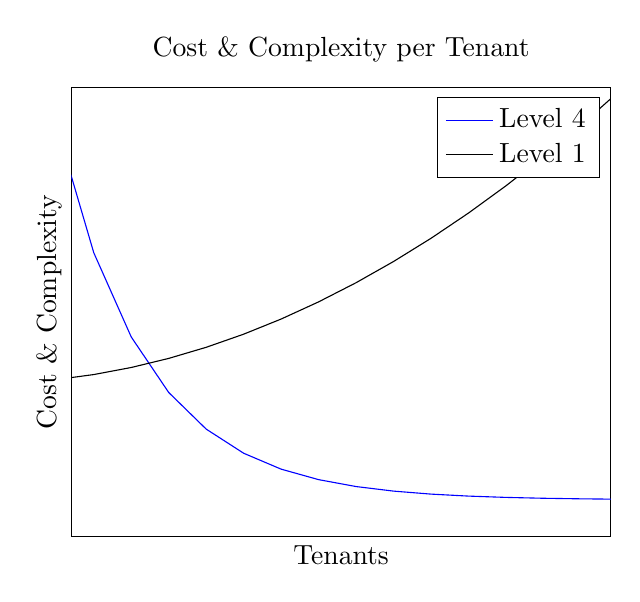
\begin{tikzpicture}
\begin{axis}[
    title={Cost \& Complexity per Tenant},
    ymajorticks=false,
    xmajorticks=false,
    xlabel={Tenants},
    ylabel={Cost \& Complexity},
    ymajorgrids=false,
    xmin=-4, xmax=2,
    grid style=dashed,
]
 
\addplot[color=blue]{exp(-x)};
	
	\addplot[color=black] {0.5(x+5)^2 + 20	};
	
\legend{Level 4, Level 1}
\end{axis}
\end{tikzpicture}

\caption{Implementation complexity per tenant}
\label{fig:imp_complexity}
\end{figure}






SaaS Maturity Level 4 is however the archetypal ideal maturity level to implement but because of its complexity is not always the first multi-tenant level developed by service providers. The 3rd maturity level is also multi-tenant enabled, but does not allow for scaling and therefore inherently contains some risks associated with it such as single point of failure and application instability. Since all tenants share this common instance, the impact of these risks are also much higher than with single-tenant applications and should therefore be kept in mind during application design. 

\section{Challenges and Requirements of multi-tenancy}
Multi-tenancy introduces many common challenges and requirements that need to be addressed in order to be implemented effectively. Common challenges include \cite{Betts2012-ad}:
\begin{itemize}
\item Partitioning \& Provisioning
\item Extensibility \& customisablity
\item Isolation \& security
\item Third Part component support
\end{itemize}

Betts \cite{Betts2012-ad} additionally outlines some of the common requirements a multi-tenant solution should consider and address from the tenants perspective inclcluding those listed above: 

\begin{itemize}
\item Availability: The application should be accessible by any tenant at any given time
\item Costs: Costs should be lower than running a dedicated hosted version of the system themselves
\item Regulatory compliance: Different tenants might require the system to comply to specific regulations, laws or standards
\item Scalability: Each tenant expects the application to meet their growing demand. Irrespective of other tenants
\end{itemize}
These requirements are very important to recognise as they can influence an service providers choice of whether or not to design their application to be multi-tenant enabled. For example service providers that do not require the scalability and availability but high levels of security and regulatory compliance might rather implement a single-tenant application that physically isolates its tenants data. 


\section{Conclusion}
This chapter took an overall look at multi-tenancy as an alternative architectural principle used for developing effective SaaS services that utilize many of the advanced capabilities offered by cloud computing. Furthermore the different levels of SaaS maturity is discussed in relation to multi-tenancy and highlights how fundamental multi-tenancy is to developing good SaaS application. Finally, the economic impact of multi-tenancy is discussed as driving force behind the choice for it to be implemented. The next chapter introduces us to the methodology used in this paper examines the specifics of how our research problem will be tackled. 